\section{Mechanical Design}

The mechanical project of the robot is completely redefined. New devices such as the chip kick and the improvement of the transmission system were developed. This robot was designed and built using CAD (Computer Aided Design) and CAM (Computer Aided Manufacturing) software, moreover extensive testing was done to validate the current project.

\begin{figure}[thpb]
	\centering
	\subfigure[]{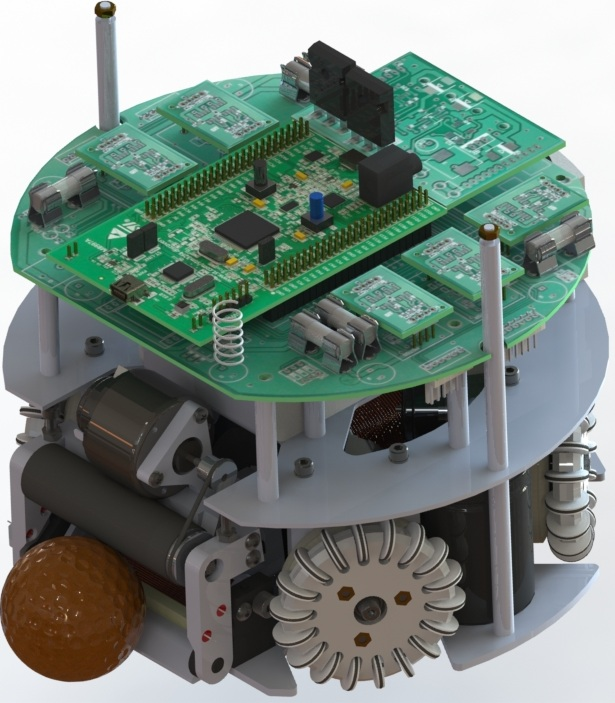
\includegraphics[width = 0.49 \textwidth]{img/modeladof2.jpg}}
	\subfigure[]{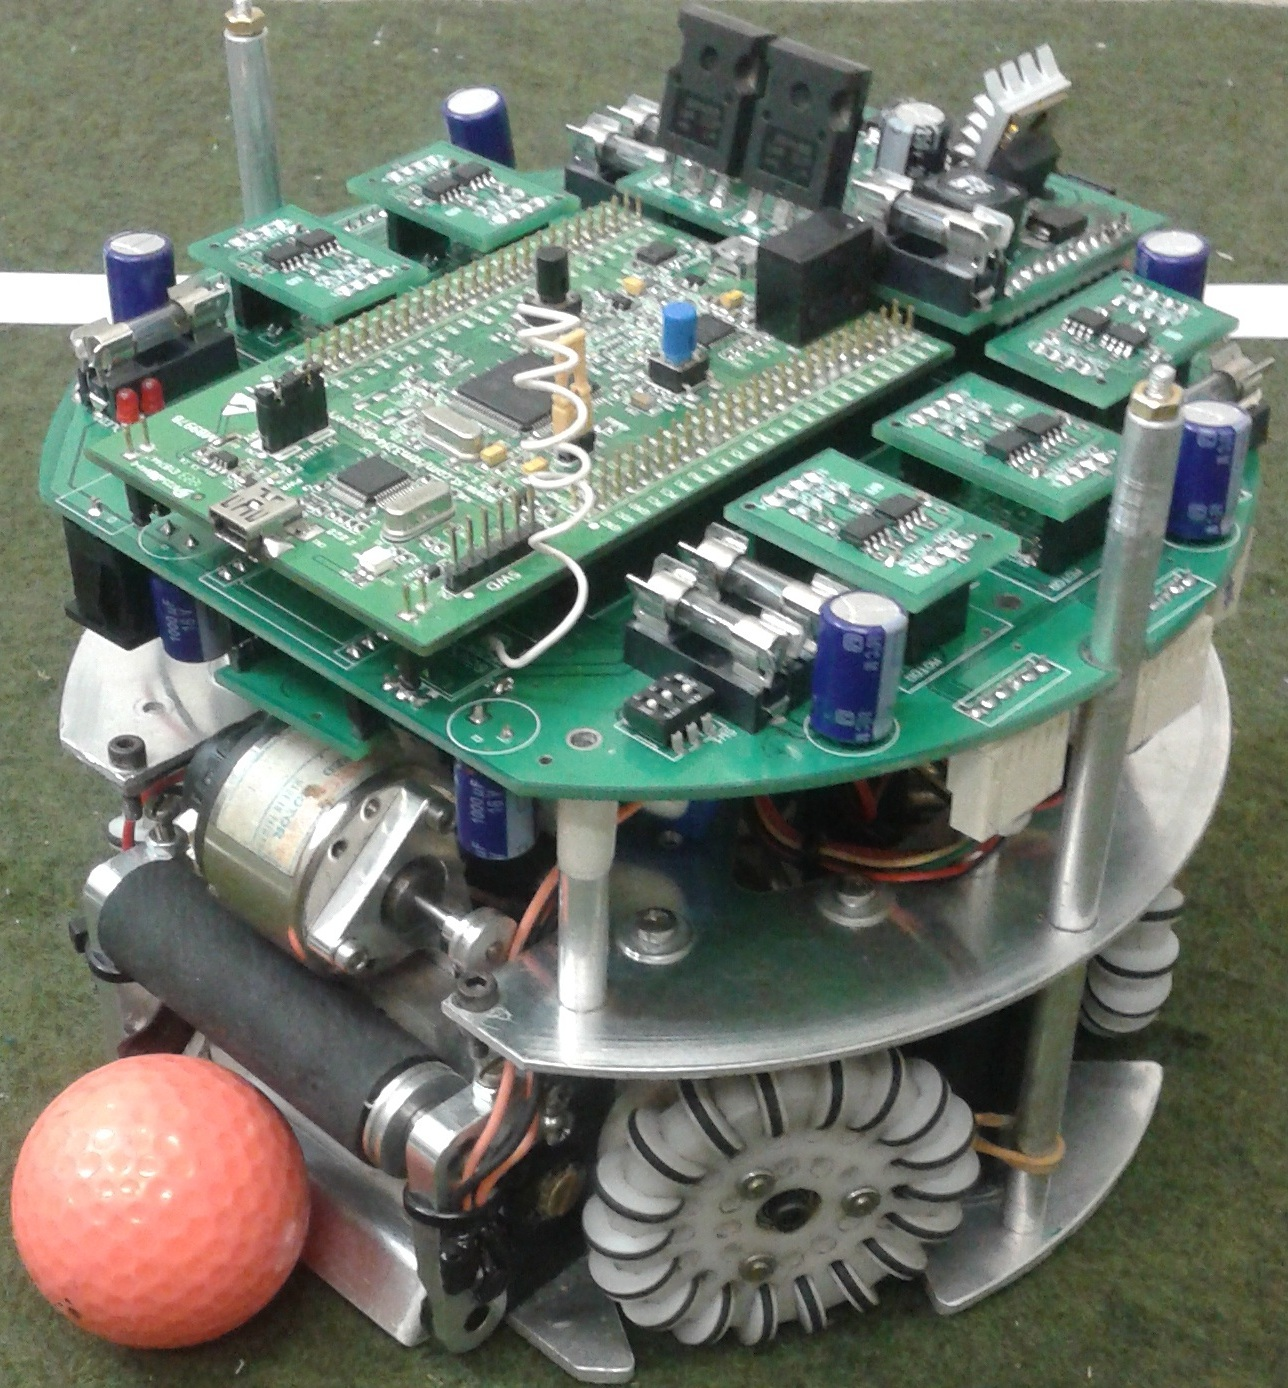
\includegraphics[width = 0.49 \textwidth]{img/realf2.jpg}}
	\caption{(a) 3D model view. (b) Robot real view.}
	\label{mec1}
\end{figure}

Most of our robot parts were CNC machined: made out of 7075 aluminium and high density polyoxymethylene (POM). The POM have some excellent properties such as: high rigidity, good impact resistance,
a non-stick characteristic and is a highly machinable material. In this way some parts of the robots, like the plunger stopping body, are more suitable to be made out of POM than aluminium. For example, the dribbler arm is a pivot-rotating mechanism, using POM eliminates the need for a bearing within the assembly.

\subsection{Dimensional Constraints}

In compliance with the SSL rules, the height of the robot is 149 mm and the maximum projection of the robot on the ground is 180 mm.

\begin{figure}[!htb]
	\centering
	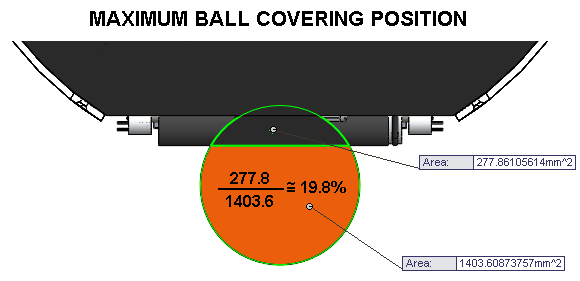
\includegraphics[width = 0.8 \textwidth]{img/20-80_rule.png}
	\caption[]{Maximum covered area of the ball}
\end{figure}

Using a CAD software we were able to measure the percentage of the ball area that was covered by the robot. The maximum percentage of ball coverage found was 19,8 \%, according to the 20/80 rule of the league. The hight of the dribbler cylinder it's also adjustable so we are able to find the optimum point for the best ball control. 

\subsection{Transmission System}

A system of internal gears was made to transmit the power of the motors to the wheels. This system has several advantages compared to traditional gear meshing. Avoiding debris entering the motors, creating a cavity to apply grease for lubrication of gears and an overall smaller size are some of them.

However there are some difficulties in the manufacture of this part, mainly due to the small size of the teeth needed to mesh with standard motor gear (the motor being used is the Hsiang Neng DC brushed motor type HN-GH35GMB). At this motor the distance between two consecutive teeth is less than 1 mm, thus it was not feasible to machine the internal gear. So it was decided for the 3D printing in ABS plastic as the manufacturing process.

Some prototyping have been done ensure accuracy and strength to the gear. The traditional fused filament deposition method for 3D printing, in geometries smaller than the filament itself, create cavernous structures that weaken the piece. Applying the stereolithography 3D printing process (when a laser beam cure a liquid resin layer by layer), we manage to achieve a higher resolution. This way we can precisely print the teeth profile, avoiding failures due to empty spots and achieving a more solid and precise component.

\begin{figure}[!htb]
	\centering
	\subfigure[]{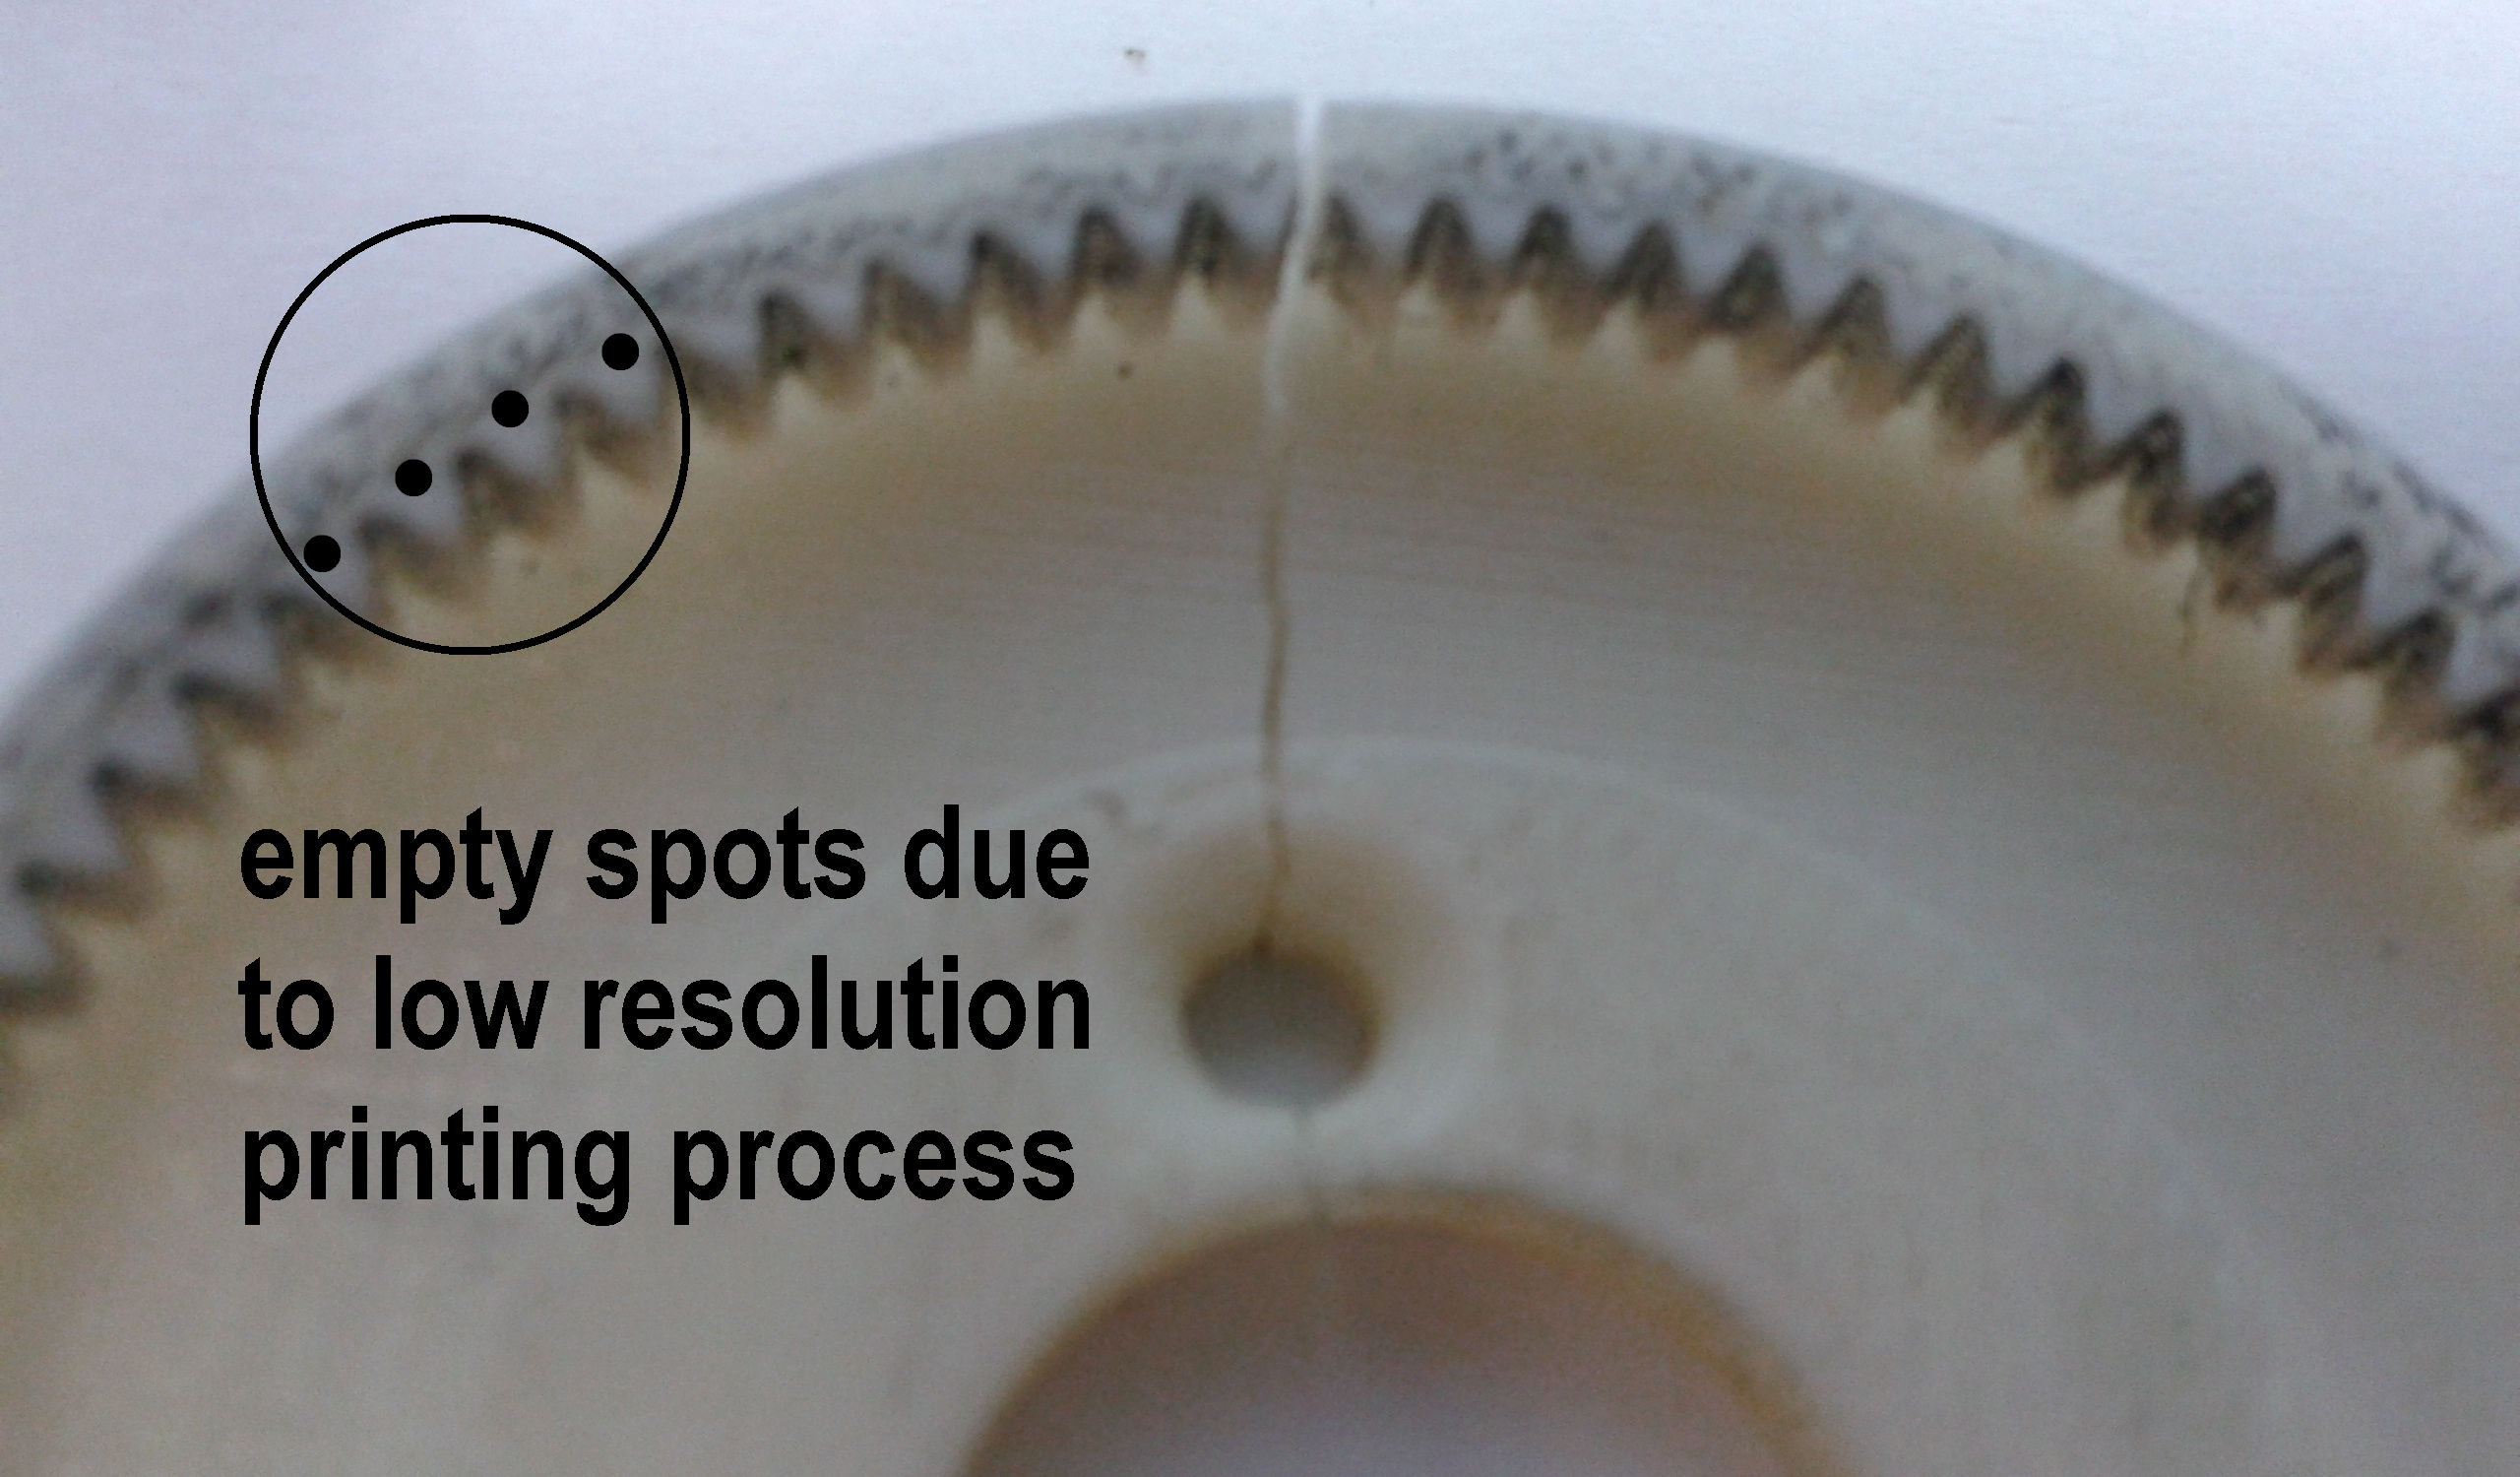
\includegraphics[width = 0.49 \textwidth]{img/gearcrack.jpg}}
	\subfigure[]{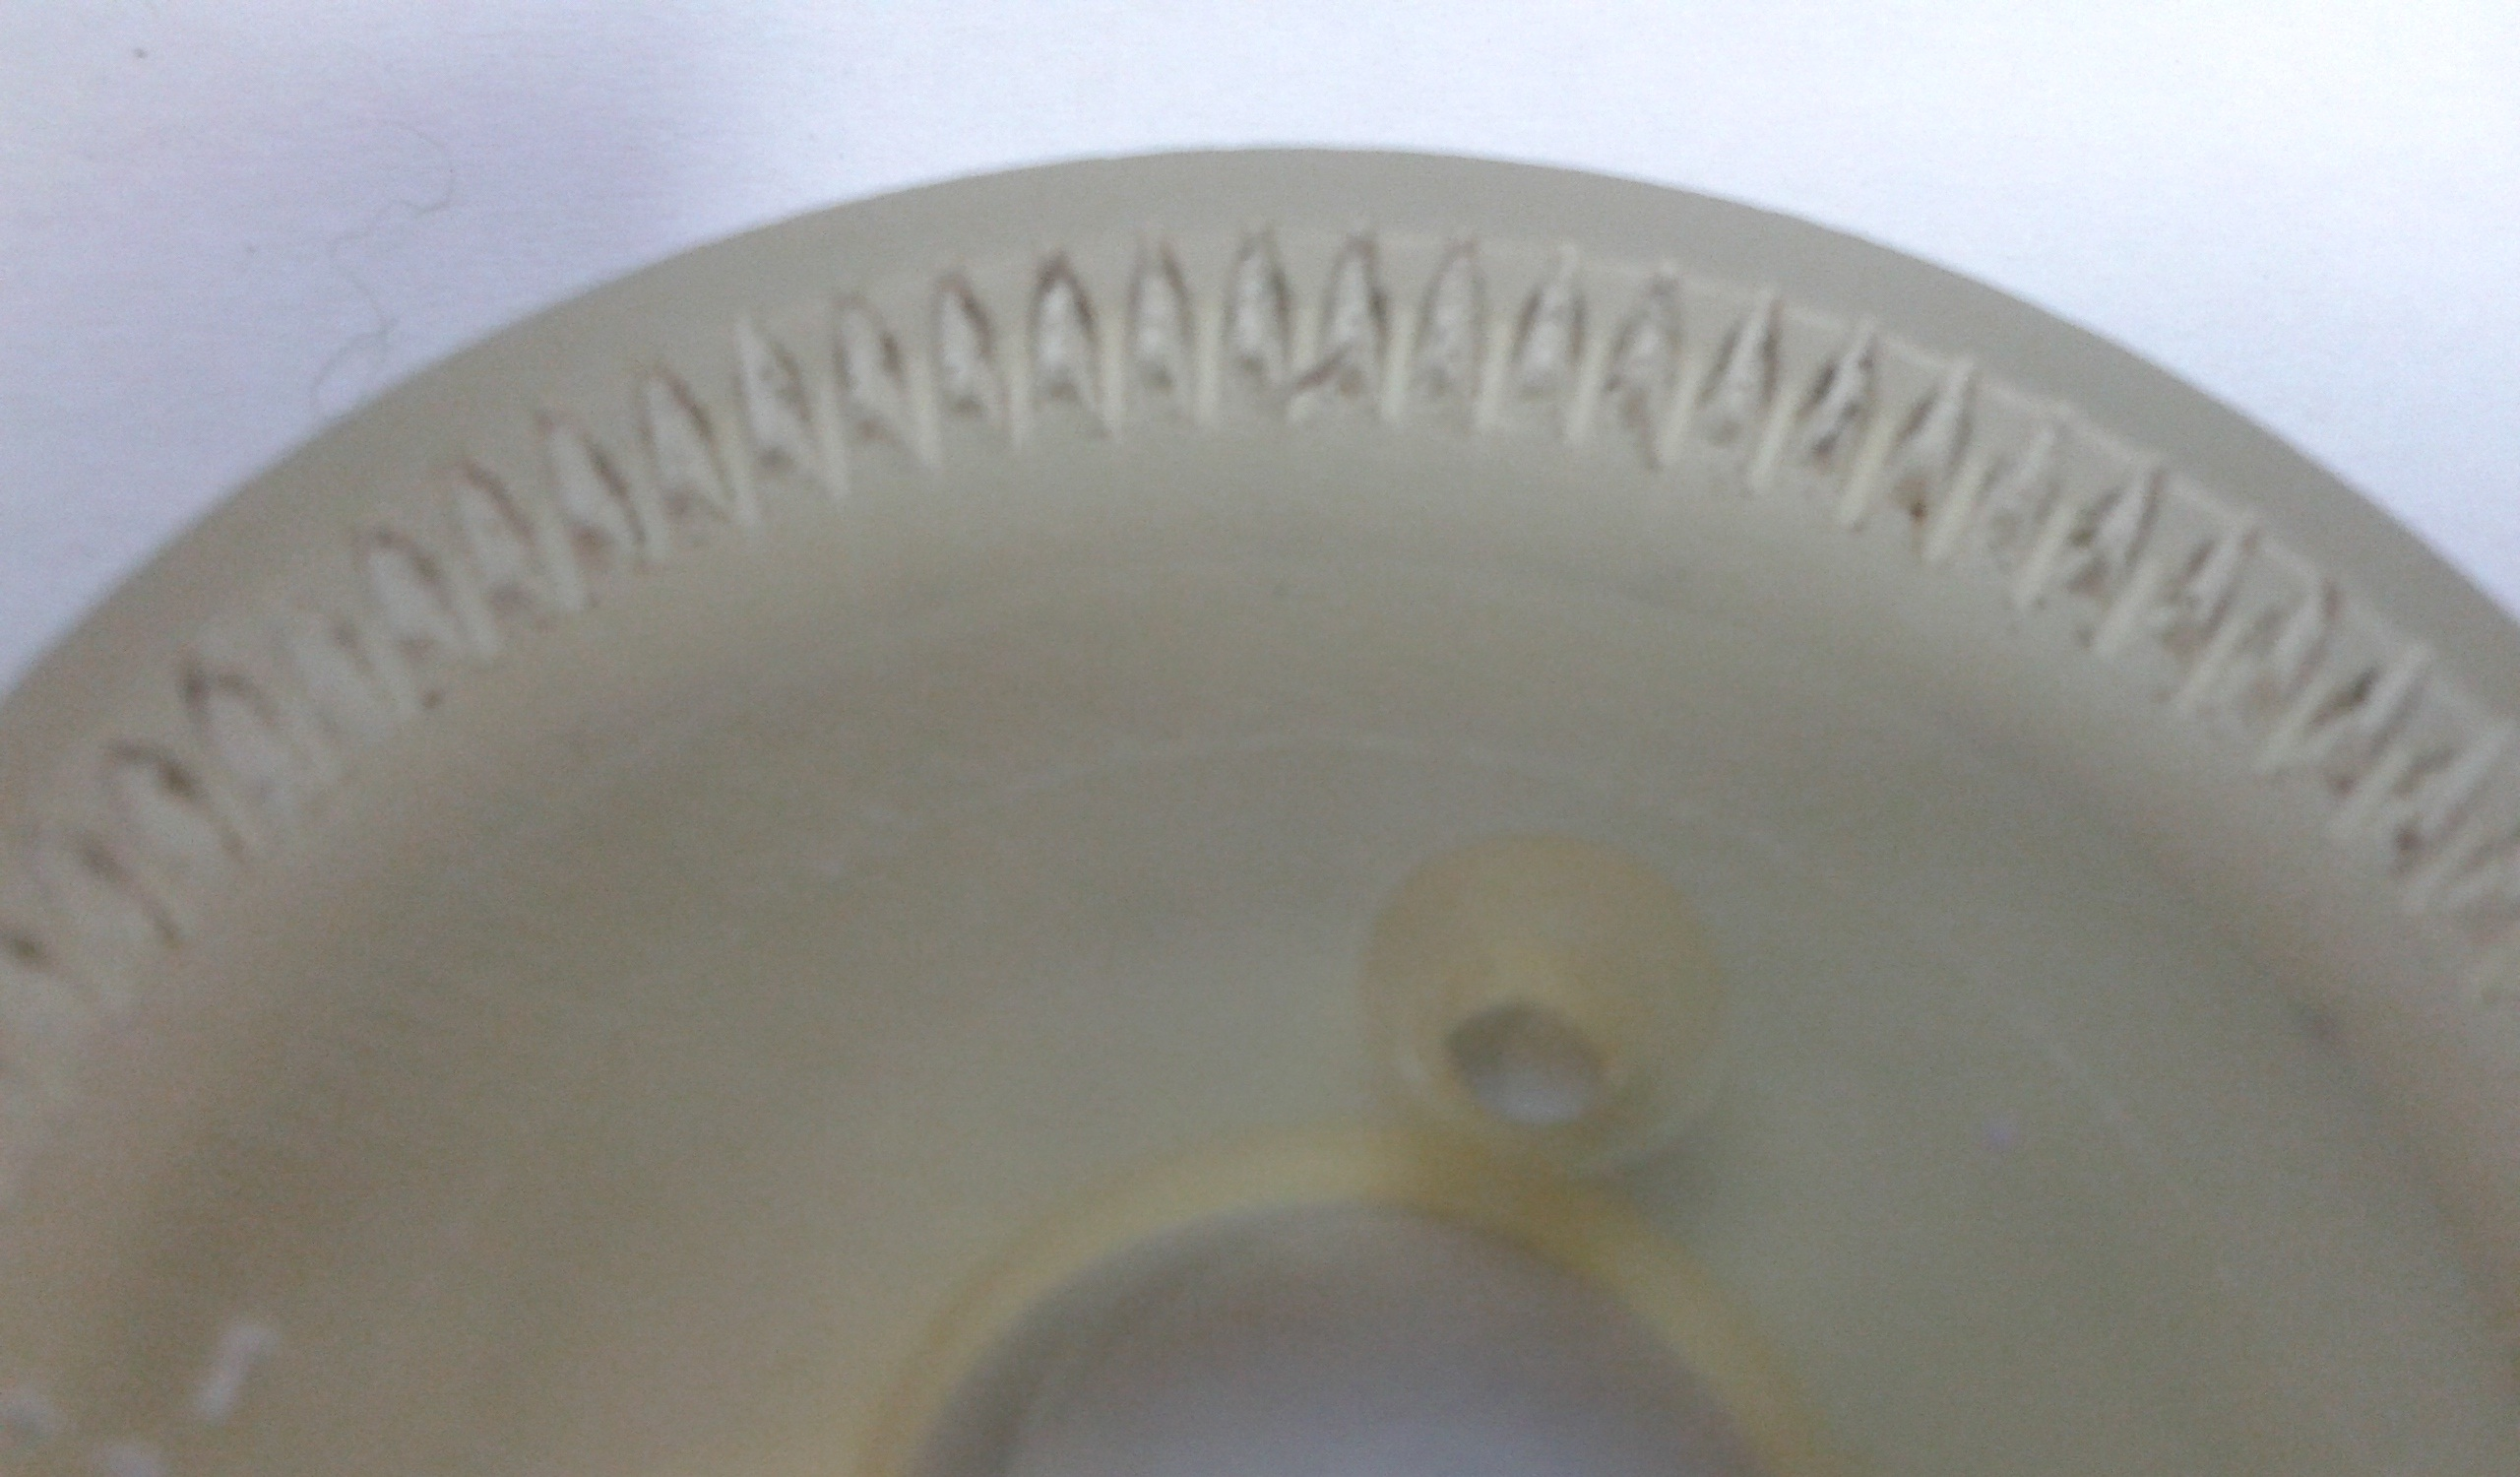
\includegraphics[width = 0.49 \textwidth]{img/gearhighresolution.jpg}}
	\caption{(a) Cracked gear (lower precision). (b) Stereolithography printed gear.}
	\label{mec3}
\end{figure}

In previously models the gears were made out of aluminium, much harder than the ABS plastic, therefore there were some concern about breaking this piece when submitted to a large load.
Full power stoppage tests were performed, locking the motor, bringing the gear to its limit. Satisfactory result were achieved making the system very reliable.

\subsection{Chip Kick}

The chip kick is based on a flat solenoid, which is mounted in a slot at the chassis (close to the ground). When activated the core of mild steel is accelerated against the rear of the chip, which revolves around it's axis and makes the ball rise. Due to the limited space, complex construction and details, we also have chosen the 3D printing as the manufacturing process.

\begin{figure}[!htb]
	\centering
	\subfigure[]{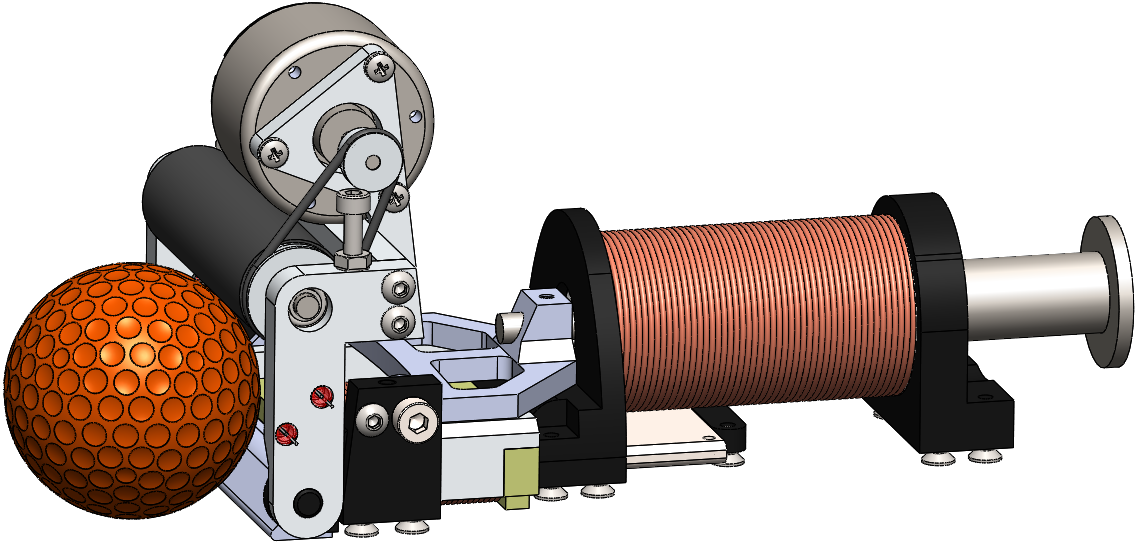
\includegraphics[width = 0.69 \textwidth]{img/fechado.png}}
	\subfigure[]{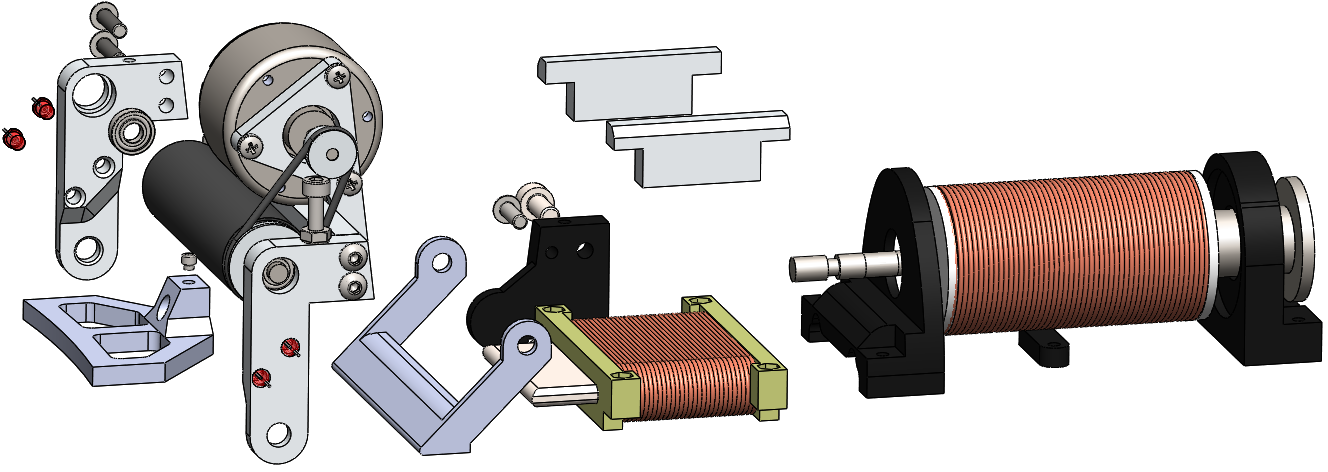
\includegraphics[width = 1 \textwidth]{img/explodida.png}}
	\caption{(a) Dribbler, chipper and kicker assembly. (b) Exploded view.}
	\label{mec4}
\end{figure}

The flat solenoid is assembled in a way that work as a guide rail for the kick plunger as well. We are using rubber-bands to pull back the chipper and kicker plungers, keeping the simplicity of the mechanism. The final dribbling/kicking mechanism is a very neat assembly and can be easily adaptable for any other chassis.
